\section{Optical Sensor Module (OS)}

The Optical Sensor Module (OS) transforms the visual activity of the analog water meter display into
a voltage. A reflective tally disk is encapsulated in the meter housing and protected by glass.
The number of rotations per
time unit corresponds to the amount of water drawn downstream.

\subsection{Requirements}

The sensor acts as an optical proximity detector. The distance between the emitter and the reflective surface
changes as the tally disc passes underneath the emitter beam.
The receiver must be able to discern this change in distance.
Furthermore, the sensor should consume as less power as possible while operating from \SI{3.3}{\volt} or
\SI{5}{\volt} supply voltage.

\subsection{Implementation}

The optical switch comprises an infrared light (\SI{940}{\nano\meter}) emitting diode with a typical forward
current of \SI{50}{\mA} and a phototransistor. In our application, the upper hatched area in
Fig.\ref{fig:osos} corresponds to the
revolving disc of the water meter totalizer.

\begin{figure}[h]
    \centering
    \includegraphics[width=0.4\textwidth]{OS/OS}
    \caption{OS - schematic}
    \label{fig:osos}
\end{figure}




\begin{table}[H]
    \centering
    \begin{threeparttable}[b]
        \begin{tabularx}{\linewidth}{ >
                    {\hsize=.25\hsize}X >
                    {\hsize=0.5\hsize}X >
                    {\hsize=.25\hsize}X  >
                    {\hsize=.5\hsize}X >
                    {\hsize=.25\hsize}X  >
                    {\hsize=3\hsize}X
            }
                  & \multicolumn{4}{c}{pin} &                                                      \\
            \cmidrule(lr){3-6}
            Id    & Net                     & Nb. & Name       & Type           & Function         \\
            \midrule
            $U_1$ & V\textsubscript{OS}     & 1   & \texttt{1} & \leftarrow     & IR diode anode   \\
            $U_1$ & \Gnd                    & 2   & \texttt{2} & \Gnd           & IR diode cathode \\
            $U_1$ & \Gnd                    & 3   & \texttt{3} &                & IR emitter       \\
            $U_1$ & \Gnd                    & 4   & \texttt{4} & \leftharpoonup & IR collector     \\
        \end{tabularx}
    \end{threeparttable}
    % \caption{WD - Pin mapping}
\end{table}

\begin{table}[H]
    \centering
    \begin{threeparttable}[b]
        \begin{tabularx}{\linewidth}{
                >{\hsize=0.25\hsize}X
                >{\hsize=1.75\hsize}X
                >{\hsize=1.5\hsize}X
                >{\hsize=0.5\hsize}X
                >{\hsize=1\hsize}X}

            Id    & Desc                          & Order Code  & Package & Note \\
            \midrule
            $U_1$ & \cite{everlight_itr9904_2010} & ITR9904/230 &         &      \\
        \end{tabularx}
    \end{threeparttable}
    % \caption{CO - BOM}
    %    \label{table:wd1}
\end{table}


\subsection{Opto Switch Drift compensation}
\label{sec:osd}
The open collector output of the phototransistor, net \cb{net}{Prx}, represents the analog reading of
the current position of the totalizer tally disc.
This value will be \textquote{high} when the reflective surface of the revolving disk does not obstruct the infrared beam emitted by the
diode in $U_8$. It will be \textquote{low} during the time when the infrared beam is reflected back to the phototransistor.
When the flow of water is low, several seconds might pass until the disc has fully traversed the region covered by the sensor.
The driver software in the master must account for this situation and filter out duplicate increments.
The question is now  which collector voltage is \textquote{high} and which is considered to be a \textquote{low}.

We observed that the collector voltage of $U_8$ is subject to drift. And indeed, the datasheet of the ITR9904 mentions several sources
of temperature dependent variables:

\begin{itemize}
    \item forward current
    \item peek emission wavelength
    \item collector power dissipation
    \item collector dark current
    \item relative collector current
\end{itemize}


This drift can be either compensate in hardware or in software. The former is not obvious because the production system can not be
easily reproduced in the lab. In addition, we suspect that the high humidity inside the gully contribute to the drift problem.

We therefore decided to implement a software compensation that is detailed in chapter \ref{sec:rsr}.
